\atsp
\begin{frame}{\ft{About}}

	\pdfpageheight 30cm

        \begin{annotatedFigure}{0pt}{0pt}
            {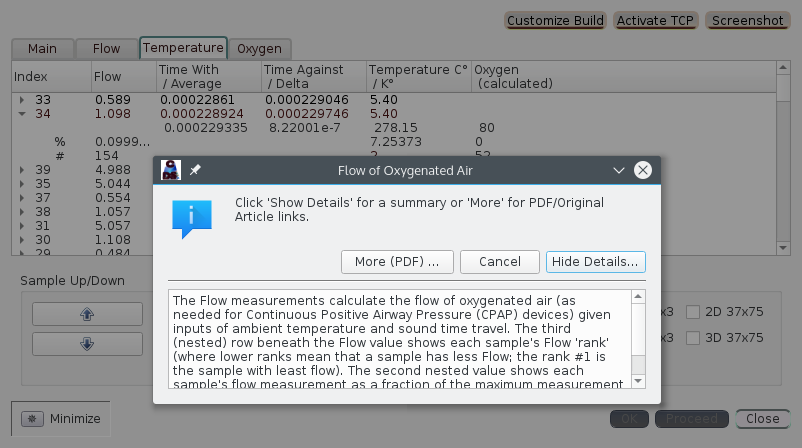
\includegraphics[scale=1]{texs/about.png}}
            
  \node [text width=13cm,align=justify,fill=logoCyan!20, draw=logoBlue, 
  draw opacity=0.5,line width=1mm, fill opacity=0.9]
   at (0.58,0.76){\textbf{Context menus also allow users to 
   obtain information and explanations about individual parts of the 
   data set, such as individual statistical parameters.  In this 
   screenshot, the user has right-clicked on a data column (Flow) and 
   has chosen a context menu action which shows, via a dialog box, 
   a precis of the quantities represented in that column and their 
   significance for the data set as a whole.}};

            \annotatedFigureBox{0.2,0.12}{0.812,0.645}{1}{0.81,0.645}%       
        \end{annotatedFigure}

\end{frame}
